\documentclass[preprint,12pt]{elsarticle}
\usepackage{amssymb}
\usepackage{lineno}
\usepackage{fixltx2e}
\usepackage{hyperref}
\usepackage{enumitem}
\usepackage{vdmlisting}
\usepackage{float}

\begin{document}

\begin{frontmatter}

\title{Modeling and simulating ERTMS/ETCS using VDM++}

%% use optional labels to link authors explicitly to addresses:
%% \author[label1,label2]{<author name>}
%% \address[label1]{<address>}
%% \address[label2]{<address>}

\author{Christian Marius Lillelund (201408354)}

\address{School of Engineering, Aarhus University}

\address{Course: E18 - Modeling of Critical Systems}

\begin{abstract}
Modeling of critical systems is an important tool in software engineering, as it allows us to design a system
from specification and verify its properties in a unambiguous way early in the development process. In this report, we use the object-oriented Vienna Development Method (VDM++) to model, simulate and verify a subset of the specifications for the safety-critical European Rail Traffic Management System (ERTMS) level 2 focusing on those properties of ERTMS that concern interlocking of tracks and safety of the trains. In ERTMS, these features are controlled by the European Train Control System (ETCS) component. With VDM++, we can perform system design analysis and model verification to catch potential faults early before the system is constructed in an implementation language like Java and deployed to a real system. We start by defining requirements and invariants based on the ERTMS/ETCS specification and then use VDM++ to design a formal model followed by model-checking. The abstract implementation of ERTMS detailed in this report provide a simple but fundamental understanding of the signaling system's behavior and how to describe its constraints.
\end{abstract}

\begin{keyword}
ERTMS \sep ETCS \sep VDM++ \sep Formal methods \sep Interlocking \sep Safety
\end{keyword}

\end{frontmatter}

\section{Introduction}
\label{S:introduction}
The railway domain was identified as a grand challenge of computing science in 2004 because it is understandable by the general public, provides useful features in terms of transportation and pose many concerns for design and controllability. One part of the challenge is improving the feasibility and capacity of modern railway as the world's population is increasing and rail traffic now moves cross borders.

The European Rail Traffic Management System (ERTMS) is a signaling and control system developed in the start 2000's to address the interoperability issues with cross-border rail traffic in Europe and lack of capacity with legacy systems. Currently many European countries have their own national stand-alone signaling and control system implemented by a certain set of rules that differ from each country. ERTMS is designed to replace the national systems to make rail transport more frictionless, improve rail capacity and more attractive to consumers. It consists of two primary parts, the European Train Control and Command System (ETCS) to govern the positions and safety of trains, known as the Interlocking (ITL), and the GSM-R radio communications system to send messages between trains and the Radio Block Center (RBC). There a three different levels of ERTMS, L1, L2 and L3. We consider L2 in this report. L2 introduces the RBC, a Eurobalise that register train movement and omits any track side signaling equipment. For a train to enter a new track section, it must requests a movement authority (MA) for that section from the RBC, which will be further explained in section X. ERTMS defines end of authority (EoA) as the point the train is allowed to move to. We consider this aspect as well.

Figure \ref{fig:ertmsoverview} shows the essential components of ERTMS level 2. The train control (EVC) requests movement authorities from the RBC over GSM-R. A typical national rail way will have multiple RBC's for each region. The RBC's communicate with a central interlocking service, that receives the physical location of trains using the Eurobalises, in order to either grant or deny movement authority to a train.

\begin{figure}[h]
	\centering
	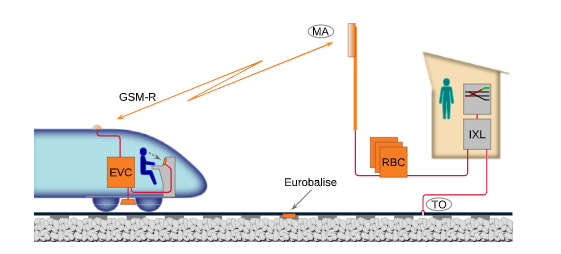
\includegraphics[width=0.8\linewidth]{ERTMS.png}
	\caption{An overview of the ERTMS/ETCS level 2 components.}
	\label{fig:ertmsoverview}
\end{figure}

\section{Requirements}
\label{S:requirements}
The purpose of the model is to design and verify the interlocking properties and operating rules of the ETCS system, a part of ERTMS. With our model we aim to show how VDM++ can we used to create and satisfy a subset of the real requirements of ETCS interlocking, abstracting away most of the physical constraints you would have in a real system and focusing on the control mechanisms you find in the RadioBlockCenter and Interlocking components, described in the introduction. Our model should demonstrate a simulated train that interacts with the control system when traversing a set of tracks, as it would in real life, while simultaneously monitoring and adhering to the safety features of the system. We address the following requirements: \\

R1: A train shall not enter a track section which is occupied by another train (same track).\\
R2: A train shall not pass a track boundary without being given a movement authority (MA) to do so.\\
R3: A train shall respect the maximum permitted speed of its current track.\\
R4: When a train has traversed half of its current track, it shall request a MA for the next track.\\
R5: Two trains cannot have a MA for the same track at the same time.\\
R6: The system shall not provide an MA for a track that is occupied by a train.\\
R7: The RBC shall not answer MA's for tracks it is not responsible for.\\
R8: The eurobalise shall report train movement to the interlocking system.\\

The requirements and the behavior of the ETCS control architecture, that we elaborate on in section \ref{S:systemarch}, are inspired from literature X and X, that describe, model and verify many of the real functional properties of ERTMS. In this report we choose a portion of these to model and test our requirements \textit{R1-R8}. UML will be used to show some of the logical VDM++ classes and their relationships. From the specification of ERTMS we can define a typical usage scenario for a train that wishes to enter a track. Given a train \textit{T1}, a track TR1 from a set of tracks (i=1,..,n), an \textit{RBC} responsible for tracks \textit{TR\textsubscript{n}}, a eurobalise \textit{Eb} mounted on the track that registers physical movement and a central interlocking service \textit{ITL}.

\begin{itemize}[noitemsep]
	\item \textit{T1} wants to enter track \textit{TR1}. \textit{T1} requests MA for \textit{TR1} from RBC.
	\item RBC contacts the ITL to verify the request.
	\item RBC grants MA to train \textit{T1} for track TR1.
	\item \textit{T1} enters track TR1.
	\item Eb registers movement and informs ITL.
\end{itemize}

This functionality will be further explored in the model architecture and design.

\section{Model architecture}
\label{S:systemarch}

The architecture of the model represents the entire system as entities, that are later defined in VDM++ as classes, that encapsulate functionality related to the individual entity. We consider the purpose of our model, that is to express and simulate several important aspects of ERMTS/ETCS, and use the primary components of such system as our entities. These can seen in figure \ref{fig:ertmscontrolarchitecture} that show a way to model the control architecture of ERTMS based in the real specification set for ERTMS level 2 detailed in X, but junction control and route guidance has been omitted.

\begin{figure}[h]
	\centering
	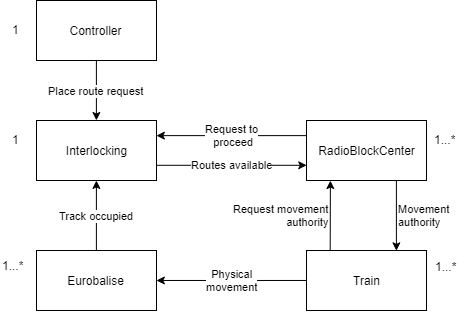
\includegraphics[width=0.8\linewidth]{ERTMSControl.png}
	\caption{The ETCS control architecture partly from the real specification.}
	\label{fig:ertmscontrolarchitecture}
\end{figure}

We shall describe the components in more detail before designing our model. The \textbf{controller} places route requests into the interlocking at certain time \textit{t} intervals. The point is to control the flow of traffic and how many routes can be available concurrently in the rail network, a way to limit congestion. A route is simply a set of tracks. \textbf{Interlocking} receives route requests and stores them in a control table containing available routes. It receives track occupation events from physical units along the track side and uses this information to update the control table with available routes. The \textbf{RadioBlockCenter} receives MA requests from trains, checks route availability and forwards these to the interlocking. RBC's are responsible for multiple tracks, i.e. a block. The \textbf{Train} sends MA requests to the RBC before entering a new track in a route. For each track, a line segment with a geographic starting and terminal point, the train must request and obtain a MA. This is also stated in the requirements. Each track has a certain speed limit, and the train must never exceed this. The \textbf{Eurobalise} registers physical movement when trains enter and leave tracks and conveys this to the interlocking. 

In a real scenario, the eurobalise sends track and speed information to passing trains and the ETCS would monitor this and eventually slow down trains, if they go too fast. We do not consider this part in our model. The ETCS architecture in figure \ref{fig:ertmscontrolarchitecture}, requirements and functionality will be used to create VDM++ classes, functions and invariants in the next section.

\section{Model design}

In this section we will review the model in VDM++ in a top-down approach and elaborate on the design choices made. The entities in our architecture are now VDM classes, types represent information state objects, and events and requests are described with operations and functions. A full class diagram can be found in Appendix A.

\subsection{Controller}
\subsection{Interlocking}
\subsection{RadioBlockCenter}
\subsection{Eurobalise}
\subsection{Train}

\section{Testing}










\begin{itemize}
\item Bullet point one
\item Bullet point two
\end{itemize}

\begin{enumerate}
\item Numbered list item one
\item Numbered list item two
\end{enumerate}

\subsection{Subsection One}

Quisque elit ipsum, porttitor et imperdiet in, facilisis ac diam. Nunc facilisis interdum felis eget tincidunt. In condimentum fermentum leo, non consequat leo imperdiet pharetra. Fusce ac massa ipsum, vel convallis diam. Quisque eget turpis felis. Curabitur posuere, risus eu placerat porttitor, magna metus mollis ipsum, eu volutpat nisl erat ac justo. Nullam semper, mi at iaculis viverra, nunc velit iaculis nunc, eu tempor ligula eros in nulla. Aenean dapibus eleifend convallis. Cras ut libero tellus. Integer mollis eros eget risus malesuada fringilla mattis leo facilisis. Etiam interdum turpis eget odio ultricies sed convallis magna accumsan. Morbi in leo a mauris sollicitudin molestie at non nisl.

\begin{table}[h]
\centering
\begin{tabular}{l l l}
\hline
\textbf{Treatments} & \textbf{Response 1} & \textbf{Response 2}\\
\hline
Treatment 1 & 0.0003262 & 0.562 \\
Treatment 2 & 0.0015681 & 0.910 \\
Treatment 3 & 0.0009271 & 0.296 \\
\hline
\end{tabular}
\caption{Table caption}
\end{table}

\subsection{Subsection Two}

Donec eget ligula venenatis est posuere eleifend in sit amet diam. Vestibulum sollicitudin mauris ac augue blandit ultricies. Nulla facilisi. Etiam ut turpis nunc. Praesent leo orci, tincidunt vitae feugiat eu, feugiat a massa. Duis mauris ipsum, tempor vel condimentum nec, suscipit non mi. Fusce quis urna dictum felis posuere sagittis ac sit amet erat. In in ultrices lectus. Nulla vitae ipsum lectus, a gravida erat. Etiam quam nisl, blandit ut porta in, accumsan a nibh. Phasellus sodales euismod dolor sit amet elementum. Phasellus varius placerat erat, nec gravida libero pellentesque id. Fusce nisi ante, euismod nec cursus at, suscipit a enim. Nulla facilisi.

Integer risus dui, condimentum et gravida vitae, adipiscing et enim. Aliquam erat volutpat. Pellentesque diam sapien, egestas eget gravida ut, tempor eu nulla. Vestibulum mollis pretium lacus eget venenatis. Fusce gravida nisl quis est molestie eu luctus ipsum pretium. Maecenas non eros lorem, vel adipiscing odio. Etiam dolor risus, mattis in pellentesque id, pellentesque eu nibh. Mauris nec ante at orci ultricies placerat ac non massa. Aenean imperdiet, ante eu sollicitudin vestibulum, dolor felis dapibus arcu, sit amet fermentum urna nibh sit amet mauris. Suspendisse adipiscing mollis dolor quis lobortis.

\begin{equation}
\label{eq:emc}
e = mc^2
\end{equation}

\section{The Second Section}
\label{S:2}

Reference to Section \ref{S:1}. Etiam congue sollicitudin diam non porttitor. Etiam turpis nulla, auctor a pretium non, luctus quis ipsum. Fusce pretium gravida libero non accumsan. Donec eget augue ut nulla placerat hendrerit ac ut mi. Phasellus euismod ornare mollis. Proin tempus fringilla ultricies. Donec pretium feugiat libero quis convallis. Nam interdum ante sed magna congue eu semper tellus sagittis. Curabitur eu augue elit.

Aenean eleifend purus et massa consequat facilisis. Etiam volutpat placerat dignissim. Ut nec nibh nulla. Aliquam erat volutpat. Nam at massa velit, eu malesuada augue. Maecenas sit amet nunc mauris. Maecenas eu ligula quis turpis molestie elementum nec at est. Sed adipiscing neque ac sapien viverra sit amet vestibulum arcu rhoncus.

Vivamus pharetra nibh in orci euismod congue. Pellentesque habitant morbi tristique senectus et netus et malesuada fames ac turpis egestas. Quisque lacus diam, congue vel laoreet id, iaculis eu sapien. In id risus ac leo pellentesque pellentesque et in dui. Etiam tincidunt quam ut ante vestibulum ultricies. Nam at rutrum lectus. Aenean non justo tortor, nec mattis justo. Aliquam erat volutpat. Nullam ac viverra augue. In tempus venenatis nibh quis semper. Maecenas ac nisl eu ligula dictum lobortis. Sed lacus ante, tempor eu dictum eu, accumsan in velit. Integer accumsan convallis porttitor. Maecenas pretium tincidunt metus sit amet gravida. Maecenas pretium blandit felis, ac interdum ante semper sed.

In auctor ultrices elit, vel feugiat ligula aliquam sed. Curabitur aliquam elit sed dui rhoncus consectetur. Cras elit ipsum, lobortis a tempor at, viverra vitae mi. Cras sed urna sed eros bibendum faucibus. Morbi vel leo orci, vel faucibus orci. Vivamus urna nisl, sodales vitae posuere in, tempus vel tellus. Donec magna est, luctus non commodo sit amet, placerat et enim.

%% The Appendices part is started with the command \appendix;
%% appendix sections are then done as normal sections
%% \appendix

%% \section{}
%% \label{}

%% References
%%
%% Following citation commands can be used in the body text:
%% Usage of \cite is as follows:
%%   \cite{key}          ==>>  [#]
%%   \cite[chap. 2]{key} ==>>  [#, chap. 2]
%%   \citet{key}         ==>>  Author [#]

%% References with bibTeX database:

\bibliographystyle{model1-num-names}
\bibliography{sample.bib}

%% Authors are advised to submit their bibtex database files. They are
%% requested to list a bibtex style file in the manuscript if they do
%% not want to use model1-num-names.bst.

%% References without bibTeX database:

% \begin{thebibliography}{00}

%% \bibitem must have the following form:
%%   \bibitem{key}...
%%

% \bibitem{}

% \end{thebibliography}


\end{document}

%%
%% End of file `elsarticle-template-1-num.tex'.
